%!TEX root = ../main.tex
%%%%%%%%%%%%%%%%%%%%%%%%%%%%%%%%%%
% Links:
%
% Difficulty: Companies: 
%%%%%%%%%%%%%%%%%%%%%%%%%%%%%%%%%%

\chapter{Jump Game}
\label{ch:can_jump}
\section*{Introduction}
In this problem we are going to investigate whether a solution exists for a game played in an array
where you are the only player and you are initially located at the first cell of it. Your goal is to
get to the last cell by jumping from a cell to another a number of times. The array contains
information about the length of the jump you can take from a cell. 

There are a number of possible solutions to this problem and in this Chapter we will discuss two of
them. In particular:
\begin{itemize}
	\item In Section \ref{can_jump:sec:backtracking} we take a look at an approach that is possibly
	 the most intuitive, where we try all possible jumps in a backtracking-like manner.
	\item In Section \ref{can_jump:sec:DFS} we will refine the solution of Section
	\ref{can_jump:sec:backtracking} into an efficient one that uses a clever insight to visit the
	cell efficiently. 
	\item Finally, in Section \ref{can_jump:sec:greedy} we will discuss an efficient and concise
	greedy solution.
\end{itemize}


\section{Problem statement}
\begin{exercise}
Write a function that takes as input  an array $I$ of non-negative integers. You are initially
positioned at the beginning of the array (at index $0$) and your goal is to jump from cell to cell
to the end of the array (cell $|I|-1$). If you are in the at index $j$ you are allowed to jump to
all cells within the following range: $[j-I_i,j+I_i]$ (each cell of the array contains the
information about the longest jump you can take from there). The function should return true if you
are able to reach the last cell of the array, false otherwise.

	\begin{example}
		\hfill \\
		Given  $I=[2,3,1,1,4]$ the function retuns \textbf{true}. You jump from cell $0$ to $1$ and
		then take a $3$ cells wide jump to the end of the array. See Figure
		\ref{fig:can_jump:example1}.
		\label{ex:can_jump_example1}
	\end{example}

	\begin{example}
		\hfill \\
		Given $I=[3,2,1,0,4]$ the function retuns \textbf{false} because it is impossible to reach
		any cells with index higher than $3$. See Figure \ref{fig:can_jump:example2}: there is not
		incoming edge for the node with label $4$.
		\label{ex:can_jump_example2}
	\end{example}
\end{exercise}

\begin{figure}
	\centering
	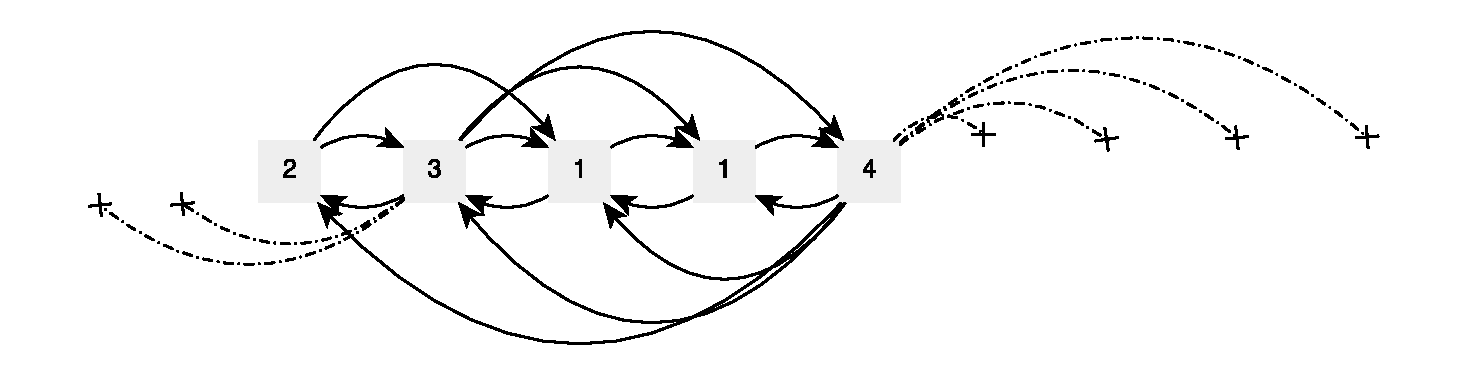
\includegraphics[width=\textwidth]{sources/can_jump/images/can_jump_example1}
	\caption[Implicit graph for the Example \ref{ex:can_jump_example1}.]
	{Visual representation (implicit graph) of the problem instance of Example
	\ref{ex:can_jump_example1}.}.
	\label{fig:can_jump:example1}
\end{figure}

\begin{figure}
	\centering
	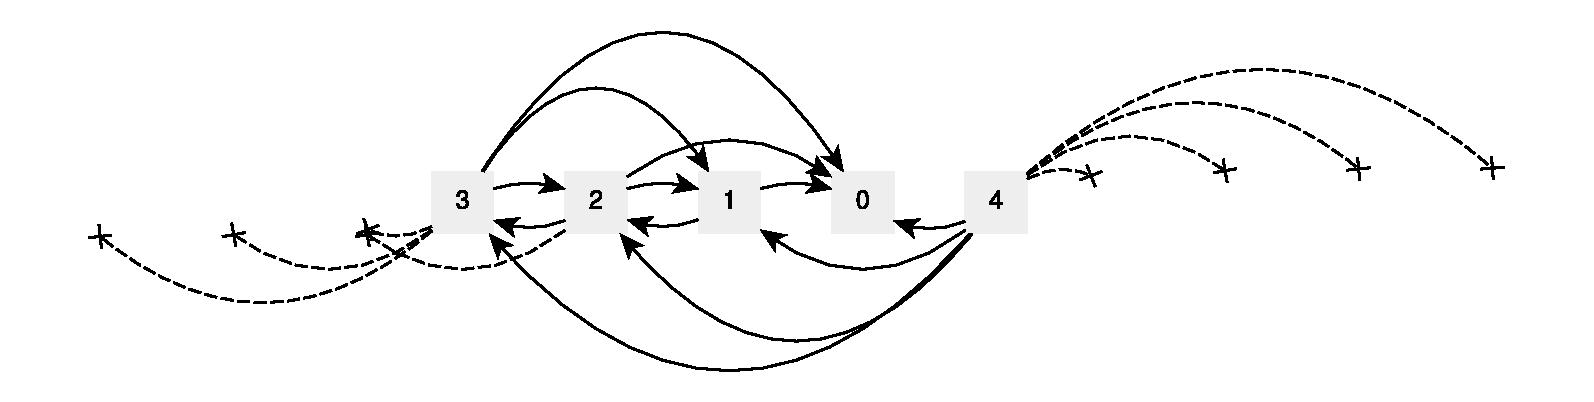
\includegraphics[width=\textwidth]{sources/can_jump/images/example2}
	\caption[Implicit graph for the Example \ref{ex:can_jump_example2}.]
	{Visual representation (implicit graph) of the problem instance of Example
	\ref{ex:can_jump_example2}.}.
	\label{fig:can_jump:example2}
\end{figure}

%\section{Clarification Questions}

%\begin{QandA}
	%\item \begin{answered}
		%\textit{}
	%\end{answered}
	
%\end{QandA}

\section{Backtracking}
\label{can_jump:sec:backtracking}
The first solution that we will investigate is one based on an idea similar to the DFS where we $I$
is treated as an implicit graph where each cell (a node) is connected to all the others cells can be
reached by jumping from it. The set of cells you can reach from a given cell $c$ is identified by
the length of the jump you can perform from $c$ which is stored within $c$ itself. The idea is to
use DFS to check whether there the last node of the graph is connected with the first one. In other
words, whether there is a path from the first to the last node. We can proceed by adopting a
recursive approach where we try to visit all the nodes that we can reach from the node we currently
occupy and to continue this process until either we have reached the last node or there is no more
jump we can try, meaning in that case, that there is no way to reach the last node (the last node is
disconnected). Because the implicit graph is not guaranteed to be acyclic, in order to make this
approach work we need to make sure is that we not jump back and forth from a cell to another in a
cycle. This can happen if for instance you jump from a cell $0$ to cell $1$ and then back to cell
$0$. In order to overcome this issue we can only perform forward jumps so that it will be impossible
to be stuck in a cycle and still manage to find an answer. When you jump to a cell $i$ from a cell
$j$ s.t. $j < i$ (you performed a forward jump) you know that you can also visit all cells $ j \leq
k \leq i$ (all the cells in between $j$ and $i$). If you only jump forward you are not going to need
to visit any cell $ j \leq k \leq i$ using backward jumps as they are visited anyway when processing
cells $j$ by performing forward jumps from it. An implementation of this idea is shown in Listing
\ref{list:can_jump1_1}. This approach is correct and it will eventually finds a solution, 	but it is
extremely inefficient. Its complexity is exponential in time as potentially the same cells are
visited over and over\footnote{Suppose $W(x)$ is the number of possible ways you can jump from
position $x$ to the end of the array at index $N$. We know that $T(N) = 1$ (the only way to jump
from cell $N$ to itself is not to jump at all). For all other cells we have that:
	\begin{align*}
		W(x) = \sum_{i=x+1}^N W(i) \\
		 = W(x+1) + \sum_{i=x+2}^N W(i) \\
		 = W(x+1) + W(x+1) \\
	  \end{align*}
	So in order to calculate $W(X)$ we need the values  $W(x+1)$ two times. The recursive tree for
	$W$ is binary and complete and has height $N$ and therefore contains $O(2^N)$ number of nodes.}
	and constant in space\footnote{if we do not consider the spaces utilized by the stack frames
	during the recursive calls, otherwise it is linear.}.

	\lstinputlisting[language=c++, caption={Exponential time solution to the \textit{jump game} problem where only forward jumps are performed.},label=list:can_jump1_1]{sources/can_jump/can_jump_solution1_1.cpp}
 
\section{DFS}
\label{can_jump:sec:DFS}
Another option for solving the cycle problem arising from the algorithm described in Section
\ref{can_jump:sec:backtracking} (this solution can be in-fact thought as an optimized backtracking)
is to keep track of the cells that we have already visited and everytime we are about to perform a
jump to a cell we first check whether that cell has been visited already in the past and if it had,
the jump is discarded and not performed. No cells is actually visited twice this way, and as a
consequence the complexity is in this case $O(|I|^2)$. In the worst-case you must check for each
cell whether all the other cells have been already visited. Listing \ref{list:can_jump1} shows an
implementation of this idea. 


\lstinputlisting[language=c++, caption={Quadratic time and linear space DFS solution to the \textit{jump game} problem using a visited array.},label=list:can_jump1]{sources/can_jump/can_jump_solution1.cpp}

Notice that one optimization from which this solution (and perhaps also Listing
\ref{list:can_jump1_1}) can benefit would be to always try to jump the longest distance possible.
Despite this would not change their asymptotic complexity, in practice this might be faster.


\section{Greedy}
\label{can_jump:sec:greedy}
There is however a much faster solution to this problem that is based on the idea that we can return
true if we can jump from the cell at index $0$ to a cell from which we can reach the end of the
array. If we apply the same reasoning to generic index $i$ we end up with basically a dynamic
programming approach that, given $G(x)$ is $1$ if you can reach the end of the array from the cell
$x$ and $0$ otherwise, is based on the following recursive formula:
\begin{equation}
	\begin{cases}
		G(|I|-1) = 1 \\
		G(x) = 1 \: \: \text{if} \: \: \exists \: y > x \:\: \text{s.t.} \:\: y < (x+I_x) \: \: \text{and} \: \:G(y) = 1\\
		\text{otherwise} \: \: G(x) = 0
	 \end{cases}
	\label{eq:can_jump:dpformula}
\end{equation}
Equation \ref{eq:can_jump:dpformula} shows that a possible implementation would start processing
cells from the last to the first and that for each element a linear time lookup for a suitable cell
$y$ might be needed. Therefore the complexity of this solution is quadratic in time. However we can
drastically lower its complexity by noticing that when processing cell $x$ all we care about is
whether the closest cell to the right from which you can reach the end of the array is reachable
from $x$. We can carry this information into a variable $m$ down from cell $|I|-1$ to cell $0$ and
update it after a cell is processed and this would effectively allow us to have a linear time
solution.

To summarize the linear time solution for this problem works as follows: We iterate the array $I$
right-to-left and for each cell $x$ we check whether we can reach $m$ jumping from $x$. If we can
then $x$ is the new leftmost cell from which we can reach the end of the array, thus $m = x$.
Otherwise we continue by processing cell $x-1$ in a similar manner. Eventually we will have
processed all cells and therefore we can return true if $m = 0$ meaning that cell $0$ is the
leftmost cell from which we can jump to location $|I|-1$, and false otherwise.
\lstinputlisting[language=c++, caption={Greedy solution where we use the fact that the DP solution described by Equation \ref{eq:can_jump:dpformula} can be optimized if we only consider if it is possible to reach the closest cell from which we can jump to the end of the array. },label=list:can_jump]{sources/can_jump/can_jump_solution2.cpp}

